\documentclass{beamer}

\mode<presentation> {
\usetheme{Madrid}
}

\beamertemplatenavigationsymbolsempty

\usepackage{pacman} % Allows you to be the best presentator ever :D

\usepackage{graphicx} % Allows including images
\usepackage{booktabs} % Allows the use of \toprule, \midrule and \bottomrule in tables
\usepackage[utf8]{inputenc}
\usepackage{float}
\usepackage{mathtools}
\usepackage{xcolor}
\usepackage{bm}
\usepackage[linesnumbered,lined,boxed,commentsnumbered]{algorithm2e}
\usepackage{scalerel}
\usepackage{setspace}
\usepackage{animate}
\usepackage{multimedia}
\usepackage{appendixnumberbeamer}

\SetAlCapNameFnt{\scriptsize}
\SetAlCapFnt{\scriptsize}

%---------------------------------------------------------------------------------------
%	TITLE PAGE
%---------------------------------------------------------------------------------------

\title[OM - 2021/22 - Lorenzo Palloni]{goa\\ (Global Optimization Animations)}
\subtitle{Optimization Methods - Global Optimization Project}
\author{Lorenzo Palloni}
\institute[]{
  University of Florence\\
  \medskip
  \textit{lorenzo.palloni@stud.unifi.it}
}
\date{\today}

\begin{document}

\begin{frame}
\titlepage % Print the title page as the first slide
\end{frame}

%---------------------------------------------------------------------------------------
%	PRESENTATION SLIDES
%---------------------------------------------------------------------------------------
%   TABLE OF CONTENTES
%---------------------------------------------------------------------------------------
%\begin{frame}
%\tableofcontents
%\end{frame}
%---------------------------------------------------------------------------------------
%---------------------------------------------------------------------------------------
\begin{frame}
\frametitle{Introduction}
  What is \textbf{goa} (Global Optimization Animations)?
  \begin{itemize}
    \item goa is a Python package that implements:
    \begin{enumerate}
      \item some problems (optimization test functions)
      \begin{itemize}
        \item Ackley function
        \item[] 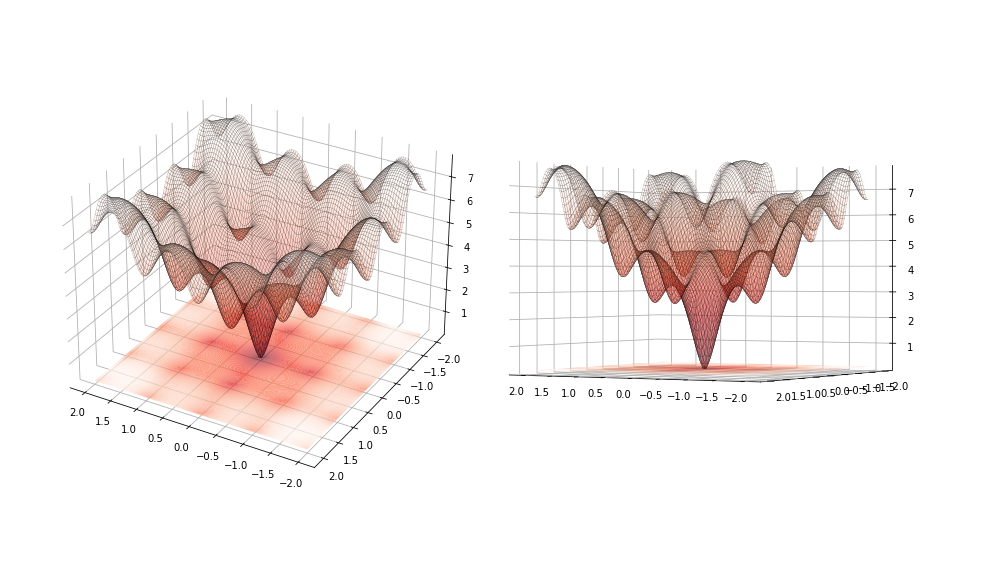
\includegraphics[width=0.3\textwidth]{figures/introduction-ackley}
        \item Rastrigin function
        \item[] 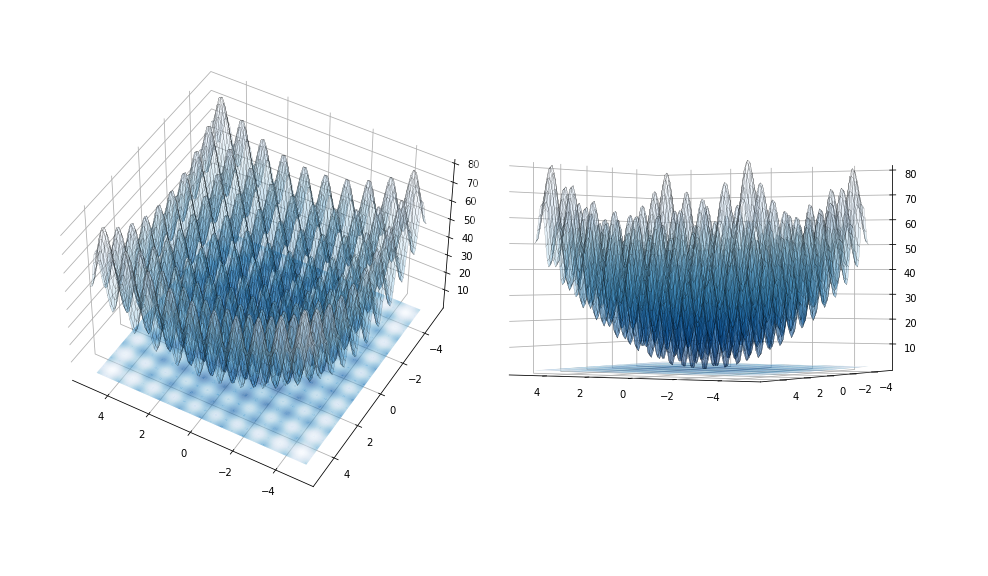
\includegraphics[width=0.3\textwidth]{figures/introduction-rastrigin}
      \end{itemize}
      \item some solutions (optimization algorithms)
      \begin{itemize}
        \item Differential Evolution \cite{de-original}
        \item Memetic Differential Evolution \cite{mde-2021}
        \item Coordinate Method with Simple Descent Direction \cite{textbook}
      \end{itemize}
    \end{enumerate}
  \end{itemize}
\end{frame}
%---------------------------------------------------------------------------------------
\begin{frame}
  \begin{block}{Definition (Ackley function)}
    $$f(x_1 \cdots x_n) = -20 exp(-0.2 \sqrt{\frac{1}{n} \sum_{i=1}^n x_i^2}) - exp(\frac{1}{n} \sum_{i=1}^n cos(2\pi x_i)) + 20 + e$$
    % $$-32 \leq x_i \leq 32$$
    $$\text{minimum at }f(0, \cdots, 0) = 0$$
  \end{block}
  \centering
  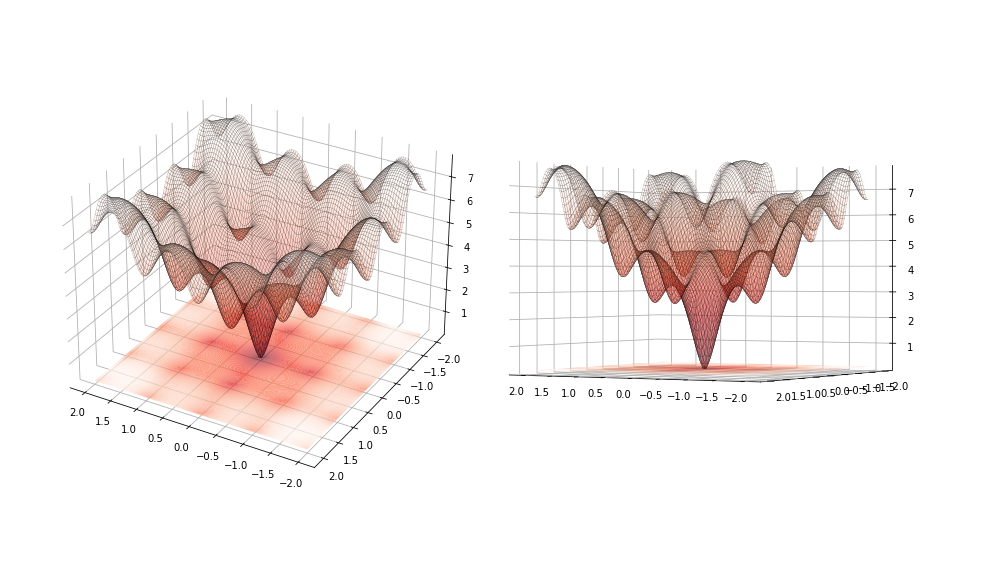
\includegraphics[width=0.8\textwidth]{figures/introduction-ackley}
\end{frame}
%---------------------------------------------------------------------------------------
\begin{frame}
  \begin{block}{Definition (Rastrigin function)}
    $$f(x_1 \cdots x_n) = 10n + \sum_{i=1}^n (x_i^2 -10cos(2\pi x_i))$$
%     $$-5.12 \leq x_i \leq 5.12$$
    $$\text{minimum at }f(0, \cdots, 0) = 0$$
  \end{block}
  \centering
  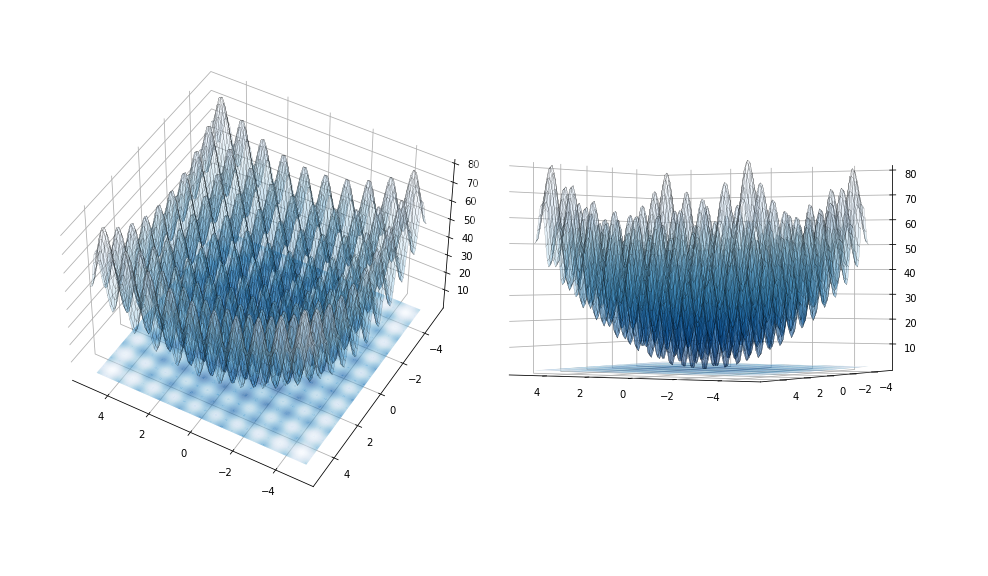
\includegraphics[width=0.8\textwidth]{figures/introduction-rastrigin}
\end{frame}
%---------------------------------------------------------------------------------------
\begin{frame}
\frametitle{Memetic Differential Evolution $vs$ Differential Evolution}
  The two algorithms differ only by the $10^{th}$ code line.
  \medskip

  \medskip
  \begin{columns}[t]
    \column{.5\textwidth}
    \centering
      \tiny
      \IncMargin{2em}
      \begin{algorithm}[H]
        \setstretch{0.5}
        \SetAlgoLined
        \KwData{$F \in (0, 2)$, $CR \in [0, 1]$}
        \ForEach{$i \in 1, \dots, p$}{
          let $ii := \mathcal{U} (1,\dots,n) $\;
          randomly choose $k_{\scaleto{1}{2pt}},k_{\scaleto{2}{2pt}},k_{\scaleto{3}{2pt}} \in \left\{ 1,\dots,p \right\} \setminus \left\{ i \right\}$\;
          let $Trial := x_{k_{\scaleto{1}{2pt}}} + F(
            x_{k_{\scaleto{2}{2pt}}} - x_{k_{\scaleto{3}{2pt}}}
          )$\;
          \For{$j \in 1,\dots,n : j \neq ii$}{
            \If{$\mathcal{U}(0, 1) < CR$}{
              let $Trial^{\scaleto{(j)}{3pt}} := x^{\scaleto{(j)}{3pt}}_{\scaleto{i}{2pt}}$\;
            }
          }
          \textcolor{purple}{let $Trial := \mathcal{L}(f, Trial)$\;}
          \If{$ f(Trial) < f(x_{\scaleto{i}{3pt}}) $}{
            let $x_{\scaleto{i}{3pt}} := Trial$\;
          }
        }
        \caption{Memetic Differential Evolution}
      \end{algorithm}
      \DecMargin{2em}
    \column{.5\textwidth}
    \centering
      \tiny
      \IncMargin{2em}
      \begin{algorithm}[H]
        \setstretch{0.5}
        \SetAlgoLined
        \KwData{$F \in (0, 2)$, $CR \in [0, 1]$}
        \ForEach{$i \in 1, \dots, p$}{
          let $ii := \mathcal{U} \left( 1,\dots,n \right) $\;
          randomly choose $k_{\scaleto{1}{2pt}},k_{\scaleto{2}{2pt}},k_{\scaleto{3}{2pt}} \in \left\{ 1,\dots,p \right\} \setminus \left\{ i \right\}$\;
          let $Trial := x_{k_{\scaleto{1}{2pt}}} + F(
            x_{k_{\scaleto{2}{2pt}}} - x_{k_{\scaleto{3}{2pt}}}
          )$\;
          \For{$j \in 1,\dots,n : j \neq ii$}{
            \If{$\mathcal{U}(0, 1) < CR$}{
              let $Trial^{\scaleto{(j)}{3pt}} := x^{\scaleto{(j)}{3pt}}_{\scaleto{i}{3pt}}$\;
            }
          }
          \textcolor{purple}{\tcp{let $Trial := \mathcal{L}(f, Trial)$}}
          \If{$ f(Trial) < f(x_{\scaleto{i}{3pt}}) $}{
            let $x_{\scaleto{i}{3pt}} := Trial$\;
          }
        }
        \caption{Differential Evolution}
      \end{algorithm}
      \DecMargin{2em}
  \end{columns}
\end{frame}
%---------------------------------------------------------------------------------------
\begin{frame}
\begin{itemize}
  \item Left example: DE reaches convergence in $38$ iterations
  \item Right example: MDE reaches convergence in $3$ iterations
\end{itemize}

\begin{itemize}
  \item[]
  \item[]
\end{itemize}

\frametitle{Animations - DE vs MDE on Ackley}
  \begin{columns}[t]
    \column{.5\textwidth}
    \centering
    \movie[showcontrols=true,height = 0.56 \textwidth,width = 1.0 \textwidth]{DE on Ackley}{movies/01-DE.mp4}
    \column{.5\textwidth}
    \centering
    \movie[showcontrols=true,height = 0.56 \textwidth,width = 1.0 \textwidth]{MDE on Ackley}{movies/01-MDE.mp4}
  \end{columns}
\end{frame}
%---------------------------------------------------------------------------------------
\begin{frame}
\begin{itemize}
  \item Left example: DE reaches convergence in $19$ iterations
  \item Right example: MDE reaches convergence in $1$ iteration
\end{itemize}

\begin{itemize}
  \item[]
  \item[]
\end{itemize}

\frametitle{Animations - DE vs MDE on Quadratic}
  \begin{columns}[t]
    \column{.5\textwidth}
    \centering
    \movie[showcontrols=true,height = 0.56 \textwidth,width = 1.0 \textwidth]{DE on Quadratic}{movies/02-DE.mp4}
    \column{.5\textwidth}
    \centering
    \movie[showcontrols=true,height = 0.56 \textwidth,width = 1.0 \textwidth]{MDE on Quadratic}{movies/02-MDE.mp4}
  \end{columns}
\end{frame}
%---------------------------------------------------------------------------------------
\begin{frame}
\frametitle{Command line interface (CLI)}
  goa provides a CLI that allows to choose:
  \begin{enumerate}
    \item problem
    \item problem bounds
    \item optimization algorithm
    \item local optimization algorithm required by memetic algorithms
    \item path for an animation of the execution of the algorithm
  \end{enumerate}
  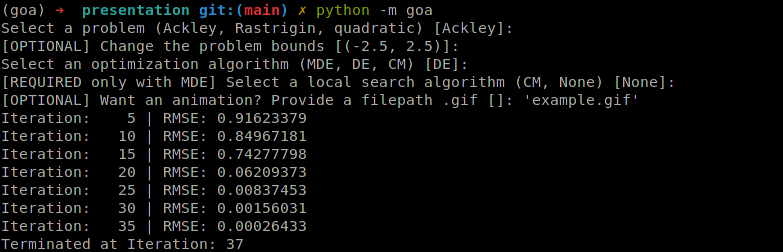
\includegraphics[width=1.0\textwidth]{figures/cli-screenshot}
\end{frame}
%---------------------------------------------------------------------------------------
\begin{frame}
\frametitle{Conclusion}

  Who would need goa?
  \begin{itemize}
    \item anyone that would like to support an explanation
    \item anyone that would like to better understand
  \end{itemize}

  \begin{itemize}
    \item[]
  \end{itemize}

  What could be improved?
  \begin{itemize}
    \item scalability (abstract classes for both global and local optimization algorithms)
    \item reproducibility (all RNGs should depend on a single random seed)
  \end{itemize}

  \begin{itemize}
    \item[]
  \end{itemize}

  Where can the implementation be found?
  \begin{itemize}
    \item \textit{https://github.com/deeplego/goa}
  \end{itemize}

\end{frame}
%---------------------------------------------------------------------------------------
\begingroup
\footnotesize
\begin{frame}
\frametitle{References}
\begin{thebibliography}{99}

\bibitem{de-original}{Storn, R. and Price, K., 1997. Differential evolution–a simple and efficient heuristic for global optimization over continuous spaces. Journal of global optimization, 11(4), pp.341-359.}
\bibitem{mde-2014}{Locatelli, M., Maischberger, M. and Schoen, F., 2014. Differential evolution methods based on local searches. Computers \& operations research, 43, pp.169-180.}
\bibitem{mde-2021}{Mansueto, P. and Schoen, F., 2021. Memetic differential evolution methods for clustering problems. Pattern Recognition, 114, p.107849.}
\bibitem{oob}{Kononova, A.V., Caraffini, F. and Bäck, T., 2020. Differential evolution outside the box. arXiv preprint arXiv:2004.10489.}
\bibitem{textbook}{Grippo, L. and Sciandrone, M., 2011. Metodi di ottimizzazione non vincolata. Springer Science \& Business Media.}

\end{thebibliography}

\end{frame}
\endgroup
%---------------------------------------------------------------------------------------
\begin{frame}[plain,c]

  {\Huge \emph{Thanks for your attention!}}

  \begin{itemize}
    \item[]
    \item[]
  \end{itemize}

  \LARGE Do you have any questions?

\end{frame}
%---------------------------------------------------------------------------------------
% \appendix
% \begin{frame}
%   \begin{centering}
%     {\Huge Backup slides}
%   \end{centering}
% \end{frame}
% %---------------------------------------------------------------------------------------

\end{document}

